\chapter{Playlists analysis}

\section{Playlist classification}
Once we have a model to classify song emotions, our next step it trying to classify playlists emotion. 
A playlist emotion can be a really useful information for a Recommender System, indeed, imagine the situation of an empty playlist, the Recommender System cannot suggest songs based on the information related to the emotion pattern inside the playlist, but what it could do is to try to understand the playlist emotion based on the title information, and then suggest songs based on this information. \par

For the emotion classification task we decided to use three artificial neural networks, with the same architecture, but trained with three different datasets: MoodyLyrics, MoodyLyrics4Q and the merged dataset. 
Fig \ref{fig:annacc} shows the different accuracies reached with each dataset. 

\begin{figure}[H]
\centering
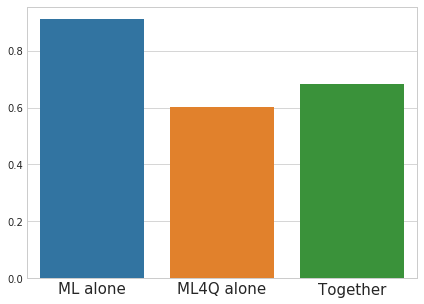
\includegraphics[width=0.7\textwidth]{./chapters/chapter5/images/ANN_accuracies.png}
\caption{5-fold ANN accuracies for each model}
\label{fig:annacc}
\end{figure}

The method we chose to classify a playlist is the following: \\
Given a \texttt{song emotion array} = [ sad\%, angry\%, happy\%, relaxed\% ] where the sum of the emotion percentage for each song is equal to one, the playlist emotion is the emotion with the maximum percentage sum over the columns. We found this approach very flexible, indeed, normalizing by the number of songs inside a playlist we obtain a probability of the emotion for that playlist. \par

However our main issue has been the absence of a labeled dataset through which compute an accuracy of our classification method. In order to overcome this problem a perfectly balanced silver standard dataset has been generated considering 40 playlist inside Spotify RecSys dataset with four really expressive titles: \textit{rage} for angry playlists, \textit{crying} for sad, \textit{party!} for happy and \textit{sleeping} for relaxed playlists. \par

The first step to classify the emotion for each song has been downloading the lyrics, and, unfortunately we noticed that we could not download the entire number of song lyrics for every playlist. Fig \ref{fig:rsongs} shows for each playlist the number of songs for which we could download the lyrics, while Fig \ref{fig:psongs} shows the percentage of available songs for each playlist. 

\begin{figure}[H]
\centering
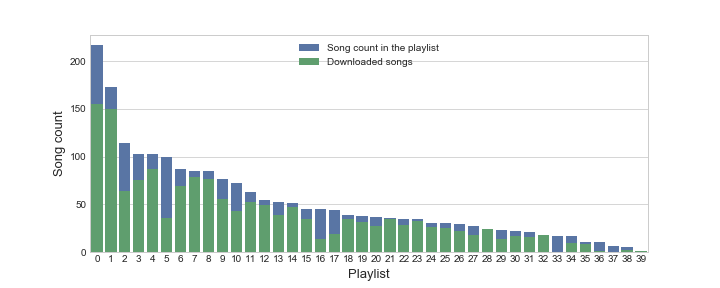
\includegraphics[width=1\textwidth]{./chapters/chapter5/images/silver_standard_available_songs.png}
\caption{Real number of available songs for playlist}
\label{fig:rsongs}
\end{figure}

\begin{figure}[H]
\centering
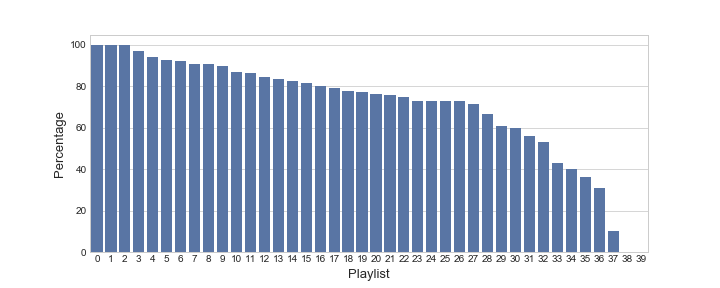
\includegraphics[width=1\textwidth]{./chapters/chapter5/images/silver_standard_percentage_available_songs.png}
\caption{Percentage of available songs for playlist}
\label{fig:psongs}
\end{figure}

Unfortunately two \textit{relaxed} playlist totally disappeared, unbalancing our silver standard.\par
We then featurized each song using the features described in Chapter 5 and classify each song using the three artificial neural networks (one trained with MoodyLyrics, one with MoodyLyrics4Q and one with the merged datasets) we previously built.\par

\subsection{Results}
Table \ref{tab:comparison2} shows the different accuracies reached classifying the playlist emotions using the method previously explained. 

\begin{table}[H]
\centering
\begin{tabular}{ |p{3cm}||p{1.5cm}|p{1.5cm}| }
 \hline
 \multicolumn{3}{|c|}{Playlist Classification Accuracy} \\
 \hline
Model trained on & With outliers & Without outliers\\
 \hline
MoodyLyrics & 24\% & 24\%\\
MoodyLyrics4Q  & 71\%    &66\%\\
Both together &   58\%  & 61\%\\
\hline
\end{tabular}
\caption{Playlist classification accuracies comparison} \label{tab:comparison2}
\end{table}

\section{Emotion patterns in playlists}







 
